\documentclass{article}
\usepackage{float,amsmath}
\usepackage{graphicx}
\usepackage{color}
\usepackage[letterpaper,margin=1in]{geometry}
\usepackage{hyperref}

%\setlength{\textwidth}{6.5in}

\begin{document}

\author{HERA}
\title{Roadmap for HERA Network Configuration and Bandwidth}
\maketitle

\section{Introduction}
HERA is an international experiment to detect and characterize the Epoch of Reionization (EOR).  The telescope is located at the South African SKA site in the Karoo
Astronomy Reserve.  This brief summarizes the overall network configuration and bandwidth for HERA as relevant to the interfaces with SKA-SA infrastructure.  HERA construction and observing are proceeding in parallel.  In late 2017 early 2018, in a major upgrade the correlator will be moved from its current location colocated with the array to the KAPB. The correlator will injest raw voltage streams at Tb speeds fed over a bundle of 96 fibers from the array to the KAPB.

\section{Current setup and KAPB move}
Figure \ref{fig:hi_level} shows the very high-level network configuration for 2017 and 2018.  In 2017 the correlator lives in the HERA 'Container' in the middle of the array.  The integrated correlator files are transferred over a dedicated fiber to processing and storage in the CMC.  The processed files are then transferred to the US, currently to a cluster at the University of Pennsylvania in Philadelphia, PA.  Over the next month or two, the CMC-based equipment will be moved to the KAPB (labelled 'b)') and the US-node will be moved to the National Radio Astronomy Observatory (NRAO) site in Socorro, NM (labelled 'c)').  The single pair of 1Ge fiber between the HERA container and the Processing node is adequate for operations through fall of 2017.

\begin{figure}[H]
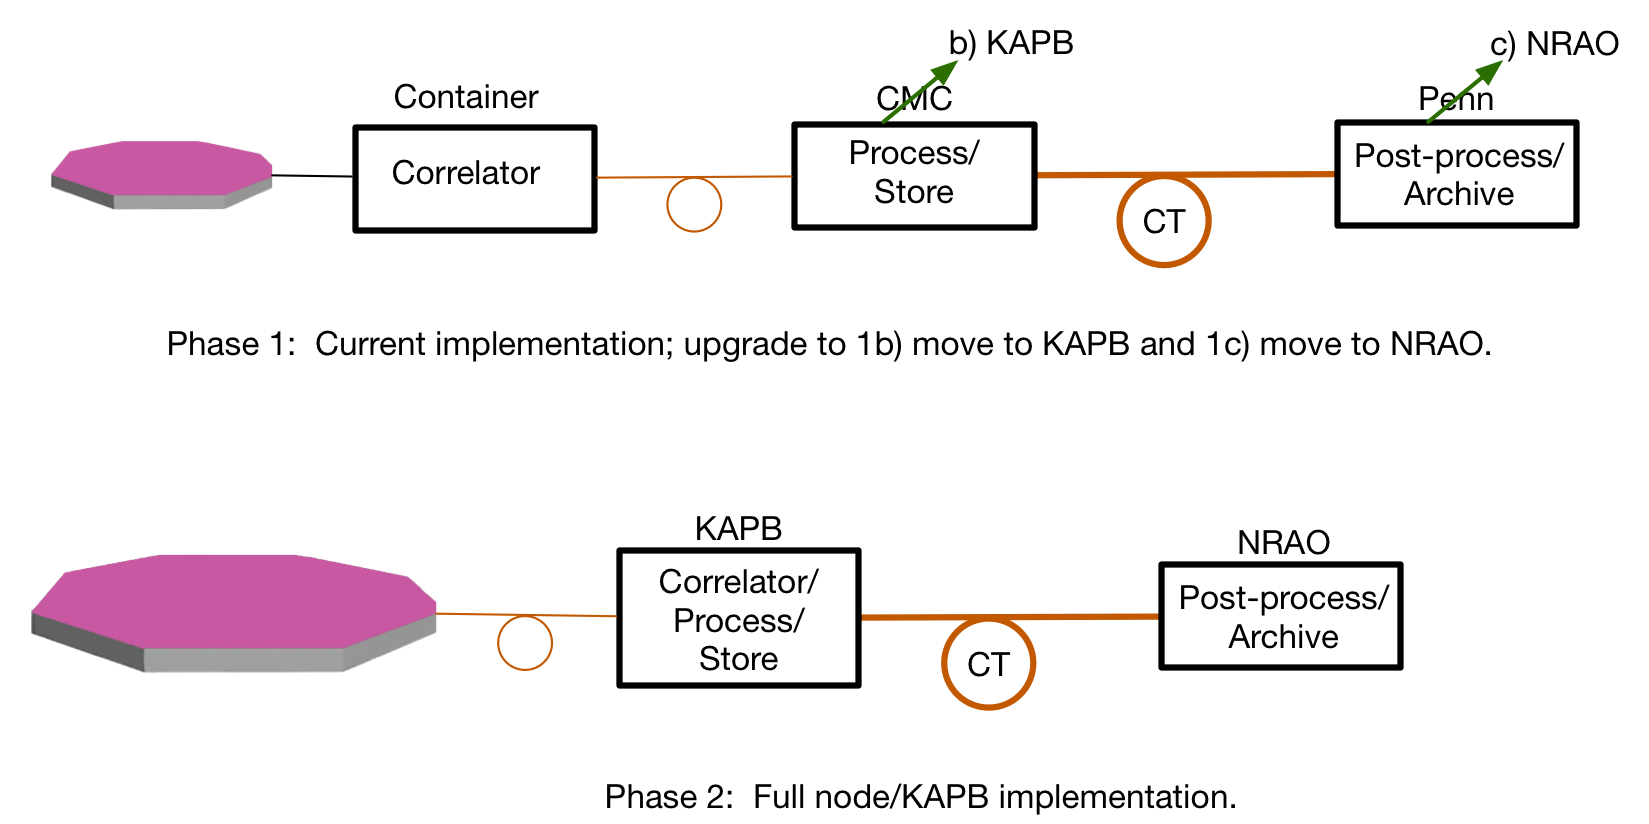
\includegraphics[width=0.8\textwidth]{network.png}
\centering
\caption{High-level organization of network.  See text for explanation.}
\label{fig:hi_level}
\end{figure}

Prior to the move of the equipment from the CMC to the KAPB, there is a desire to change the network configuration to accommodate both new site and new HERA changes in the current network.  There is no strict requirement that this need happen before that move, however it allows the network change to be tested before a major hardware relocation.  When the equipment is relocated to the KAPB additional storage will be added to the system, as well as upgrading the switches.

The proposed network arrangement is shown in Figure \ref{fig:net_org}.  The primary requirements for the current system that will take us through the middle of 2018 are:
\begin{enumerate}
\item login portal for access from the internet
\item access to the KAT network for integration with CAM
\item a dedicated fiber pair between the HERA container and Processing cluster (currently CMC, soon KAPB)
\item 32 reserved IP addresses on the KAT network
\item data rate to the US of 200Mbps by mid 2017 growing to 400Mbps by mid 2018
\end{enumerate}

\begin{figure}[H]
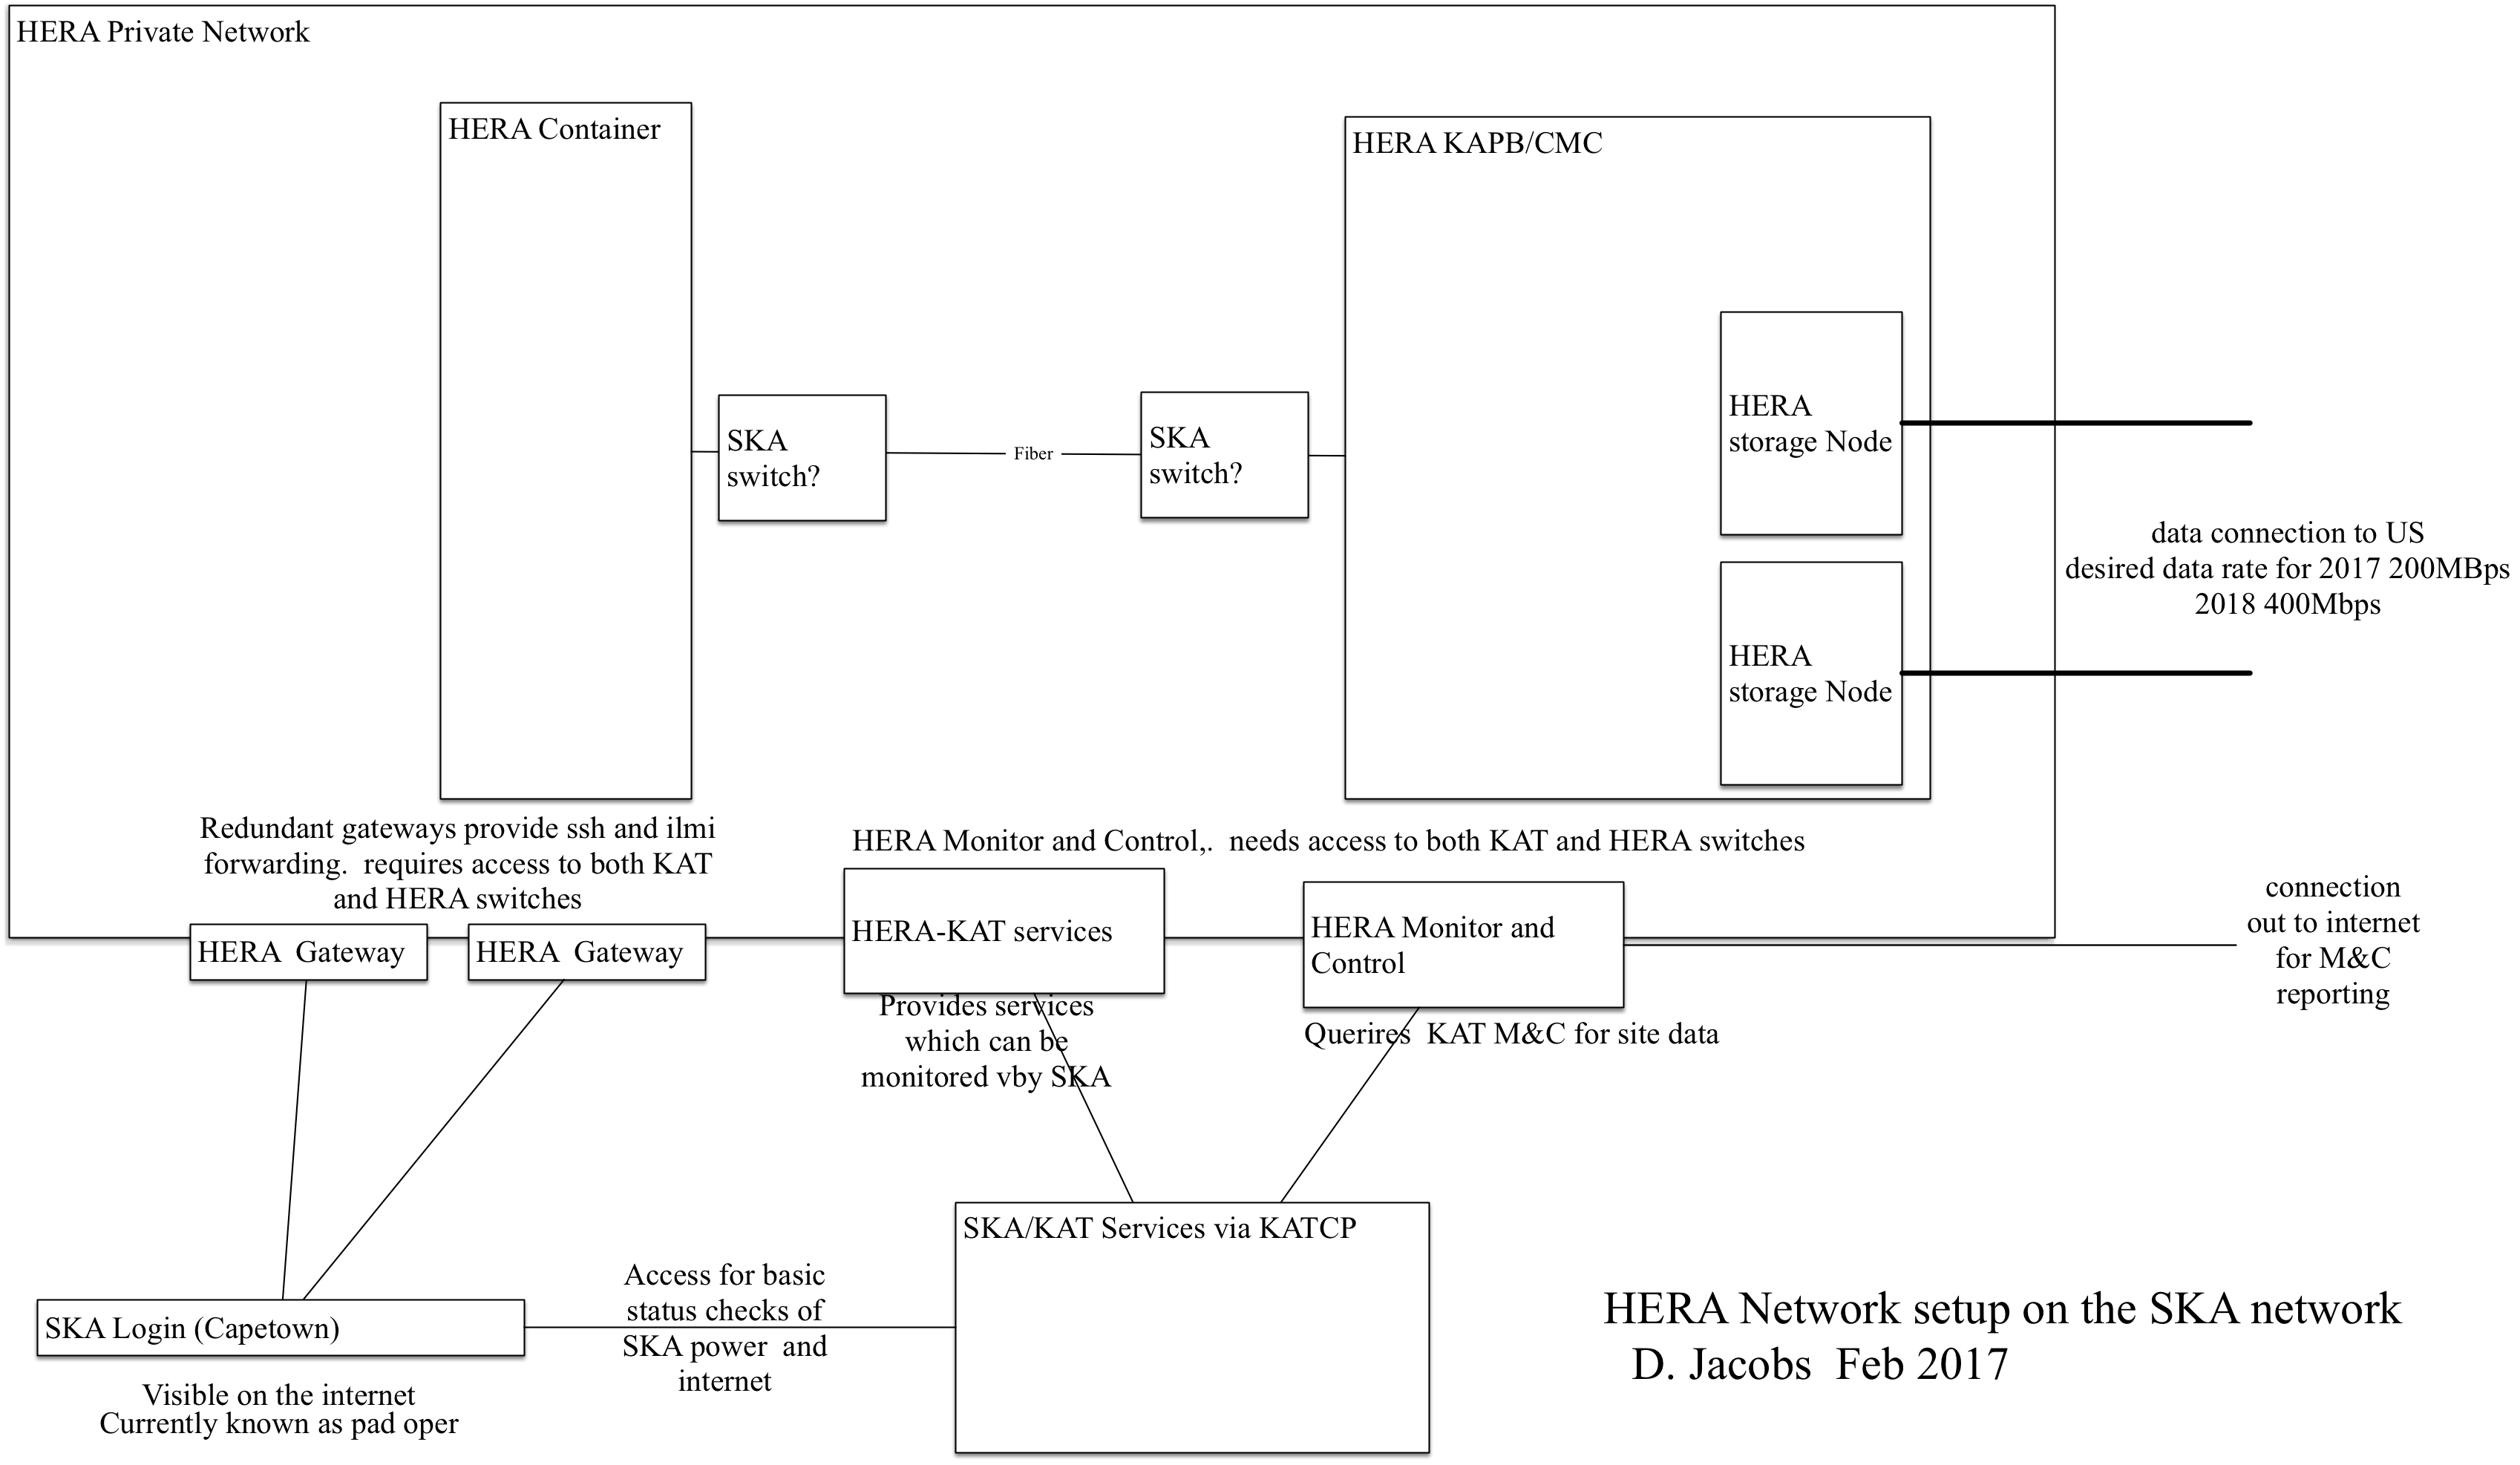
\includegraphics[width=0.8\textwidth]{HERA_2017_network_organization.png}
\centering
\caption{Proposed networking diagram.}
\label{fig:net_org}
\end{figure}

\section{Data Rate}
HERA currently records at a data rate of 200Mbps and in 2018 will increase to 1.5Gbps. Currently the average bandwidth to the US is 60Mbps so we extract a small fraction of data for transfer. This limits analysis capabilities and means only a small fraction of data exists in multiple copies.  Even moving data at the rate of 60Mbps causes conflict with SKA SA staff internet use, so copies to the US are limited to night time hours.  

The desired data rate to support current operations is 200Mbps, and the target for mid 2018 is 400Mbps.

\end{document}